\section{Additional mechanism analyses}
\label{sup:analyses}

The accompanying generated tables expand the main-paper evidence along five
axes: the complete Admission-loss grid; rejection-objective controls; shared
versus isolated ownership; complete-expression, canonical-text, and generic
Admission interventions; and sensitivity to the relative Admission margin.
These are mechanism or calibration analyses unless explicitly marked as a
preregistered held-out contrast.

% Generated by paper/scripts/make_main_tables.py.
\begin{table*}[t]
\centering
\caption{Cumulative implementation ladder.  It documents how the released
system was assembled; it is not an equal-supervision or equal-capacity causal
comparison.}
\label{tab:supp-cumulative-routes}
\scriptsize
\setlength{\tabcolsep}{4pt}
\begin{tabular}{lrrrrrr}
\toprule
Route & Test5$\uparrow$ & FPR95$\downarrow$ & Elig. recall$\uparrow$ & Elig. $n\downarrow$ & Active (K) & Cumulative (K) \\
\midrule
Frozen base & 72.16 & 51.21 & -- & -- & 0 & 0 \\
+ complete-expression Ranking & -- & -- & -- & -- & 50.2 & 50.2 \\
+ static Admission$^{\dagger}$ & -- & -- & -- & -- & 0 & 50.2 \\
+ learned Admission & 74.24 & -- & 99.69 & 69.5 & 268.2 & 318.3 \\
+ isolated Abstention (ARROW-U2) & 74.24 & 47.02 & 99.69 & 69.5 & 84.0 & 402.3 \\
\bottomrule
\end{tabular}
\parbox{0.97\textwidth}{\scriptsize Percentages except eligible count and
parameter columns. Admission+Ranking and the full system have bitwise-identical
queries, selected boxes, and localization records. $^\dagger$Static Admission
is validation-only, so no held-out endpoint is assigned.}
\end{table*}


% Generated by paper/scripts/make_main_tables.py.
\begin{table*}[t]
\centering
\caption{Per-split and per-seed Ref validation results for every trajectory with a sealed three-seed forward. Split columns average the three seeds; seed columns are pooled Val3 micro Acc@0.5. These are validation-only mechanism results.}
\label{tab:supp-ref-breakdown}
\scriptsize
\setlength{\tabcolsep}{3.2pt}
\begin{tabular}{llcccccc}\toprule
Block & ID & RefCOCO & RefCOCO+ & RefCOCOg & s17 & s42 & s73\\\midrule
Admission & A1 & 65.87 & 72.75 & 80.58 & 71.17 & 71.32 & 71.67 \\
Admission & A3 & 66.70 & 74.40 & 80.68 & 72.24 & 72.49 & 72.50 \\
Admission & A4 & 66.65 & 74.43 & 80.32 & 72.38 & 72.28 & 72.35 \\
Admission & A5 & 66.66 & 74.32 & 80.68 & 72.23 & 72.46 & 72.40 \\
Ownership & O0 & 66.81 & 74.38 & 80.64 & 72.42 & 72.42 & 72.49 \\
Ownership & O1 & 66.72 & 74.25 & 80.63 & 72.33 & 72.32 & 72.40 \\
Ownership & O2 & 66.65 & 74.40 & 80.64 & 72.40 & 72.38 & 72.36 \\
Ownership & O3 & 66.66 & 74.32 & 80.68 & 72.23 & 72.46 & 72.40 \\
\bottomrule\end{tabular}
\parbox{0.97\textwidth}{\scriptsize A0/A2 are absent here because only deployment parity and a single-seed static route were sealed; reporting copied three-seed values would overstate the available evidence.}
\end{table*}


% Generated by paper/scripts/make_main_tables.py.
\begin{table}[t]
\centering
\caption{Strong RefCOCO localization scale check. These standard split
scores are not the five-split Test5 endpoint and are not an ARROW superiority
contrast.}
\label{tab:supp-strong-baseline}
\scriptsize
\setlength{\tabcolsep}{4.2pt}
\begin{tabular}{lrrr}\toprule
Evidence source & Val & TestA & TestB\\\midrule
MM-GDINO-T 5e (model zoo) & 89.50 & 91.40 & 86.60 \\
Local epoch-5 frozen replay & 89.33 & 91.27 & 86.42 \\
\bottomrule\end{tabular}
\parbox{0.96\columnwidth}{\scriptsize P@1 at IoU$\geq0.5$ (\%). The
published row is a model-zoo reference, not a local forward. The local row is
recomputed from the exact frozen epoch-5 state (SHA-256 prefix
\texttt{2ec6fbc0}). Its training configuration evaluated Val/TestA/TestB
every epoch, so it is a retrospective replay rather than virgin held-out
evidence.}
\end{table}


% Generated by paper/scripts/make_main_tables.py.
\begin{table*}[t]
\centering
\caption{Capacity-controlled transfer on the frozen MM-GDINO-T RefCOCO e5
trunk.  Val is mechanism-only; TestAB is the micro average of TestA and TestB.
Strict columns use Strict-TN2031.  The published MMDetection reference is
Val/TestA/TestB=89.5/91.4/86.6; it is not a local-forward row.}
\label{tab:supp-strong-ownership}
\scriptsize
\setlength{\tabcolsep}{3.2pt}
\begin{tabular}{lrrrrrrrrr}
\toprule
Route & Seed & Val & TestA & TestB & TestAB & FPR95$\downarrow$ & AUROC$\uparrow$ & AUPR$\uparrow$ & Grad. cos.\\
\midrule
Native e5 & -- & 89.330 & 91.267 & 86.418 & 88.969 & 88.282 & 66.412 & 66.080 & -- \\
Shared-128 & 17 & 89.339 & 91.267 & 86.438 & 88.979 & 83.703 & 67.537 & 65.300 & -0.0633 \\
Shared-128 & 42 & 89.339 & 91.267 & 86.398 & 88.960 & 85.032 & 66.591 & 63.561 & +0.0082 \\
Shared-128 & 73 & 89.339 & 91.285 & 86.418 & 88.979 & 87.592 & 62.502 & 59.384 & -0.0111 \\
Shared-Wide & 17 & 89.330 & 91.285 & 86.438 & 88.988 & 84.146 & 68.024 & 66.481 & -0.0178 \\
Shared-Wide & 42 & 89.367 & 91.267 & 86.438 & 88.979 & 83.653 & 68.498 & 67.404 & +0.0324 \\
Shared-Wide & 73 & 89.330 & 91.267 & 86.418 & 88.969 & 83.259 & 68.167 & 66.260 & +0.0118 \\
Isolated & 17 & 89.339 & 91.267 & 86.457 & 88.988 & 84.884 & 67.600 & 66.478 & zero \\
Isolated & 42 & 89.339 & 91.267 & 86.398 & 88.960 & 81.979 & 68.226 & 67.025 & zero \\
Isolated & 73 & 89.339 & 91.285 & 86.418 & 88.979 & 85.771 & 65.623 & 64.376 & zero \\
\bottomrule
\end{tabular}
\par\medskip
\textbf{Shared-trunk gradient trajectory}\par\smallskip
\begin{tabular}{lrrrrr}
\toprule
Route & Seed & U25 & U50 & U100 & U150\\
\midrule
Shared-128 & 17 & +0.030 & +0.042 & -0.247 & -0.063 \\
Shared-128 & 42 & -0.016 & -0.004 & +0.004 & +0.008 \\
Shared-128 & 73 & -0.014 & -0.008 & -0.005 & -0.011 \\
Shared-Wide & 17 & +0.022 & +0.026 & -0.053 & -0.018 \\
Shared-Wide & 42 & +0.102 & +0.115 & +0.012 & +0.032 \\
Shared-Wide & 73 & +0.046 & +0.043 & +0.024 & +0.012 \\
\bottomrule
\end{tabular}
\parbox{0.98\textwidth}{\scriptsize All learned rows use the fixed
preregistered endpoint, FP32, clip 0.1, and AdamW with zero weight decay. Rank and rejection
have separate optimizer states in every arm; Shared arms intentionally point
those states at the same trunk parameters. Shared-128 has 50,308 parameters
and 49,536 MAC/query; Shared-Wide has 100,362 and 99,424; Isolated has 100,358
and 98,816. Confidence never selects a query or box. Each Strict bootstrap
replicate recomputes its positive q05.}
\end{table*}


% Generated by paper/scripts/make_main_tables.py.
\begin{table*}[t]
\centering
\caption{Strong-trunk continuation stress test.  The original e5 result is the
reference in Tab.~\ref{tab:supp-strong-ownership}; this block runs only the
capacity-matched Shared-Wide/Isolated pair at the fixed U150 endpoint.}
\label{tab:supp-strong-e6-ownership}
\scriptsize
\setlength{\tabcolsep}{4pt}
\begin{tabular}{lllrrrr}
\toprule
Frozen trunk & Owner & Seed ID & TestA & TestB & TestAB & FPR95$\downarrow$\\
\midrule
e6 PosCtrl & Shared-Wide & A & 91.126 & 86.477 & 88.923 & 83.358 \\
e6 PosCtrl & Shared-Wide & B & 91.126 & 86.457 & 88.914 & 82.915 \\
e6 PosCtrl & Shared-Wide & C & 91.126 & 86.438 & 88.904 & 83.013 \\
e6 PosCtrl & Isolated & A & 91.126 & 86.438 & 88.904 & 83.210 \\
e6 PosCtrl & Isolated & B & 91.126 & 86.477 & 88.923 & 82.373 \\
e6 PosCtrl & Isolated & C & 91.126 & 86.438 & 88.904 & 84.244 \\
e6 TN10 & Shared-Wide & A & 91.232 & 86.791 & 89.128 & 67.258 \\
e6 TN10 & Shared-Wide & B & 91.250 & 86.791 & 89.137 & 66.913 \\
e6 TN10 & Shared-Wide & C & 91.232 & 86.791 & 89.128 & 67.110 \\
e6 TN10 & Isolated & A & 91.232 & 86.791 & 89.128 & 68.193 \\
e6 TN10 & Isolated & B & 91.250 & 86.791 & 89.137 & 67.159 \\
e6 TN10 & Isolated & C & 91.232 & 86.771 & 89.118 & 70.606 \\
\bottomrule
\end{tabular}
\par\medskip
\begin{tabular}{llrrrr}
\toprule
Frozen trunk & Probe horizon & Mean cosine & $P(\cos<0)$ & q05 & Minimum\\
\midrule
e6 PosCtrl & all audit milestones & +0.0103 & 46.9 & -0.2483 & -0.3538 \\
e6 PosCtrl & final endpoint & -0.0453 & 58.3 & -0.1820 & -0.2422 \\
e6 TN10 & all audit milestones & +0.0543 & 53.1 & -0.4704 & -0.6727 \\
e6 TN10 & final endpoint & -0.0763 & 66.7 & -0.5162 & -0.5596 \\
\bottomrule
\end{tabular}
\par\smallskip
\begin{tabular}{lrrr}
\toprule
Frozen trunk & Isolated$-$Shared REC [CI] & FPR95 reduction [CI] & Holm-IUT $p$\\
\midrule
e6 PosCtrl & -0.003 [-0.009, 0.000] & -0.181 [-1.923, 1.118] & 1.0000 \\
e6 TN10 & -0.003 [-0.009, 0.000] & -1.559 [-2.925, -0.304] & 1.0000 \\
\bottomrule
\end{tabular}
\parbox{0.98\textwidth}{\scriptsize Percentages except gradient statistics.
Positive FPR95 reduction favors Isolated.  The same image-cluster draw is used
for both trunks, owners, and all seeds; every replicate recomputes each
positive q05.  TN10 deepens the negative tail but does not improve Isolated
REC, and its rejection interval favors Shared-Wide.}
\end{table*}


% Generated by paper/scripts/make_main_tables.py.
\begin{table*}[t]
\centering
\caption{MM-GDINO-T pretrained-trunk ownership replay.  The trunk has broad
grounding pretraining but no RefCOCO-specific full-model fine-tuning; only the
capacity-matched Shared-Wide/Isolated pair is trained at fixed U150.}
\label{tab:supp-pretrain-ownership}
\scriptsize
\setlength{\tabcolsep}{3.2pt}
\begin{tabular}{llrrrrr}
\toprule
Owner & Seed & Test5 & TestAB & FPR95$\downarrow$ & AUROC$\uparrow$ & AUPR$\uparrow$\\
\midrule
Shared-Wide & A & 56.734 & 53.413 & 92.664 & 59.630 & 59.589 \\
Shared-Wide & B & 56.741 & 53.404 & 90.596 & 60.129 & 58.950 \\
Shared-Wide & C & 56.569 & 53.330 & 89.759 & 59.994 & 58.939 \\
Isolated & A & 56.605 & 53.367 & 91.925 & 59.331 & 60.001 \\
Isolated & B & 56.699 & 53.367 & 92.319 & 54.726 & 53.914 \\
Isolated & C & 56.456 & 53.246 & 90.842 & 57.521 & 57.678 \\
\bottomrule
\end{tabular}
\par\smallskip
\begin{tabular}{lrrrrr}
\toprule
Owner & RefCOCO A & RefCOCO B & RefCOCO+ A & RefCOCO+ B & RefCOCOg\\
\midrule
Shared-Wide & 59.319 & 46.791 & 59.012 & 48.381 & 63.213 \\
Isolated & 59.230 & 46.771 & 58.883 & 48.381 & 63.046 \\
\bottomrule
\end{tabular}
\par\smallskip
\begin{tabular}{lrrrrr}
\toprule
Probe horizon & $n$ & Mean cosine & $P(\cos<0)$ & q05 & Minimum\\
\midrule
all milestones & 96 & +0.0510 & 38.5 & -0.2064 & -0.2743 \\
final endpoint & 24 & -0.0015 & 45.8 & -0.1691 & -0.1792 \\
\bottomrule
\end{tabular}
\par\smallskip
\begin{tabular}{lrr}
\toprule
Endpoint & Isolated$-$Shared [95\% CI] & Interpretation\\
\midrule
Test5 & -0.095 [-0.129, -0.061] & Shared-Wide higher\\
TestAB & -0.056 [-0.104, -0.013] & Shared-Wide higher\\
FPR95 reduction & -0.689 [-2.340, 0.365] & interval crosses zero\\
\bottomrule
\end{tabular}
\parbox{0.98\textwidth}{\scriptsize Percentages except gradient statistics.
FPR95 reduction is Shared-Wide minus Isolated, hence positive values favor
Isolated. Statistics use 5,000 paired image-cluster bootstrap replicates; every
FPR95 replicate recomputes each route/seed positive q05. The five Test5 split
means are three-seed means. Isolated has no cross-task autograd path.}
\end{table*}


% Generated by paper/scripts/make_main_tables.py.
\begin{table*}[t]
\centering
\caption{Direct pre-Stage-B GroundingDINO parent ownership replay.  Native,
Shared-Wide, and Isolated use identical frozen candidates and the
full-expression mean score; learned routes use the fixed endpoint.}
\label{tab:supp-original-parent-ownership}
\scriptsize
\setlength{\tabcolsep}{3.2pt}
\begin{tabular}{llrrrrr}
\toprule
Owner & Seed & Test5 & TestAB & FPR95$\downarrow$ & AUROC$\uparrow$ & AUPR$\uparrow$\\
\midrule
Native & -- & 39.533 & 40.588 & 89.660 & 55.756 & 54.977 \\
Shared-Wide & A & 42.714 & 42.792 & 90.596 & 58.244 & 56.923 \\
Shared-Wide & B & 42.885 & 42.885 & 93.796 & 52.636 & 52.133 \\
Shared-Wide & C & 43.773 & 43.406 & 91.581 & 57.660 & 56.300 \\
Isolated & A & 40.993 & 41.815 & 90.497 & 57.848 & 56.294 \\
Isolated & B & 40.715 & 41.574 & 93.599 & 52.956 & 51.346 \\
Isolated & C & 41.661 & 42.346 & 93.944 & 52.718 & 52.347 \\
\bottomrule
\end{tabular}
\par\smallskip
\begin{tabular}{lrrrrr}
\toprule
Owner & RefCOCO A & RefCOCO B & RefCOCO+ A & RefCOCO+ B & RefCOCOg\\
\midrule
Native & 41.188 & 39.921 & 36.360 & 38.249 & 40.898 \\
Shared-Wide & 45.277 & 40.530 & 40.983 & 38.835 & 46.692 \\
Isolated & 43.362 & 40.301 & 38.450 & 38.399 & 43.220 \\
\bottomrule
\end{tabular}
\par\smallskip
\begin{tabular}{lrrrrr}
\toprule
Probe horizon & $n$ & Mean cosine & $P(\cos<0)$ & q05 & Minimum\\
\midrule
all milestones & 96 & +0.0541 & 35.4 & -0.1005 & -0.3240 \\
final endpoint & 24 & +0.0118 & 50.0 & -0.2288 & -0.3240 \\
\bottomrule
\end{tabular}
\par\smallskip
\begin{tabular}{lrr}
\toprule
Endpoint & Isolated$-$Shared [95\% CI] & Interpretation\\
\midrule
Test5 & -2.001 [-2.269, -1.735] & Isolated fails non-inferiority\\
TestAB & -1.116 [-1.482, -0.741] & Isolated fails non-inferiority\\
FPR95 reduction & -0.689 [-2.046, 0.182] & interval crosses zero\\
\bottomrule
\end{tabular}
\parbox{0.98\textwidth}{\scriptsize Percentages except gradient statistics.
FPR95 reduction is Shared-Wide minus Isolated. Statistics use 5,000 paired image-cluster
replicates and recompute every positive q05. The direct-parent raw-query owners
have 100,362/100,358 parameters; the existing frozen-base integrated owners have
83,971/83,969.  This table alone is not a cross-stage contrast; the strict
same-100k-head adapted replay is reported in the next table.}
\end{table*}


% Generated by paper/scripts/make_main_tables.py.
\begin{table*}[t]
\centering
\caption{Strict same-100k-head adapted-trunk replay and direct-parent difference-in-differences.}
\label{tab:supp-same-head-stage-axis}
\scriptsize
\setlength{\tabcolsep}{3.2pt}
\begin{tabular}{llrrrrr}
\toprule
Owner & Seed & Test5 & TestAB & FPR95$\downarrow$ & AUROC$\uparrow$ & AUPR$\uparrow$\\
\midrule
Native & -- & 72.046 & 65.690 & 50.222 & 83.067 & 81.547 \\
Shared-Wide & A & 72.172 & 65.802 & 46.677 & 83.289 & 80.008 \\
Shared-Wide & B & 72.198 & 65.876 & 46.923 & 84.264 & 82.442 \\
Shared-Wide & C & 72.137 & 65.792 & 47.218 & 84.597 & 82.796 \\
Isolated & A & 72.130 & 65.811 & 47.070 & 81.211 & 75.517 \\
Isolated & B & 72.127 & 65.802 & 46.036 & 84.373 & 82.487 \\
Isolated & C & 72.091 & 65.792 & 46.135 & 84.763 & 82.823 \\
\bottomrule
\end{tabular}
\par\smallskip
\begin{tabular}{lrrrrr}
\toprule
Probe horizon & $n$ & Mean cosine & $P(\cos<0)$ & q05 & Minimum\\
\midrule
all milestones & 96 & +0.0306 & 47.9 & -0.4471 & -0.6234 \\
final endpoint & 24 & -0.0335 & 58.3 & -0.1745 & -0.3747 \\
\bottomrule
\end{tabular}
\par\smallskip
\begin{tabular}{lrrl}
\toprule
Parent$\rightarrow$adapted DiD & Effect & 95\% CI & Decision\\
\midrule
Test5 ownership effect & +1.948 & [1.686, 2.208] & excludes zero \\
TestAB ownership effect & +1.094 & [0.718, 1.462] & excludes zero \\
FPR95-reduction ownership effect & +1.215 & [-0.113, 2.631] & crosses zero \\
\bottomrule
\end{tabular}
\parbox{0.98\textwidth}{\scriptsize Adapted-trunk Isolated$-$Shared:
Test5 -0.053 [-0.095, -0.011],
TestAB -0.022 [-0.104, 0.054];
FPR95 reduction +0.525 [-0.444, 1.100].
All values are percentages or percentage points except cosine.  The 5,000
paired image-cluster replicates use the same draw across parent/adapted trunks, owners,
and seeds and recompute every positive q05.}
\end{table*}


% Generated by paper/scripts/make_main_tables.py.
\begin{table*}[t]
\centering
\caption{Zero-update rank-dataset probe on the same RefCOCO-e5 trunk and U150
shared checkpoints.  Only the rank batch changes; each route/seed reuses the
same eight formal D3 confidence batches and sealed queue.  All values are
three-seed means except the lower seed table.}
\label{tab:supp-cross-dataset-probe}
\scriptsize
\setlength{\tabcolsep}{2.6pt}
\begin{tabular}{llrrrrrrrr}
\toprule
Owner & Rank data & Cos. & Sign-conf. & $\lVert g_R\rVert$ & $\lVert g_C\rVert$ & Native P@1 & Rank loss & Top1 margin & Oracle gap\\
\midrule
Shared-128 & RefCOCO & +0.0714 & 0.4857 & 0.0372 & 0.0206 & 89.45 & 0.4380 & 0.6899 & 0.6273 \\
Shared-128 & RefCOCO+ & +0.0739 & 0.4851 & 0.0344 & 0.0206 & 74.48 & 0.4133 & 0.5551 & 0.3949 \\
Shared-128 & RefCOCOg & +0.0792 & 0.4851 & 0.0402 & 0.0206 & 82.68 & 0.4925 & 0.6500 & 0.5215 \\
Shared-Wide & RefCOCO & +0.0260 & 0.4916 & 0.0384 & 0.0501 & 89.45 & 0.4376 & 0.6899 & 0.6273 \\
Shared-Wide & RefCOCO+ & +0.0235 & 0.4929 & 0.0342 & 0.0501 & 74.48 & 0.4127 & 0.5551 & 0.3949 \\
Shared-Wide & RefCOCOg & +0.0282 & 0.4902 & 0.0412 & 0.0501 & 82.68 & 0.4919 & 0.6500 & 0.5215 \\
\bottomrule
\end{tabular}
\par\smallskip
\begin{tabular}{llrrr}
\toprule
Owner & Rank data & seed17 cosine & seed42 cosine & seed73 cosine\\
\midrule
Shared-128 & RefCOCO & +0.1100 & +0.0993 & +0.0051 \\
Shared-128 & RefCOCO+ & +0.0752 & +0.1395 & +0.0069 \\
Shared-128 & RefCOCOg & +0.0756 & +0.1535 & +0.0086 \\
Shared-Wide & RefCOCO & +0.0087 & +0.0739 & -0.0045 \\
Shared-Wide & RefCOCO+ & +0.0075 & +0.0946 & -0.0316 \\
Shared-Wide & RefCOCOg & +0.0036 & +0.0867 & -0.0057 \\
\bottomrule
\end{tabular}
\parbox{0.98\textwidth}{\scriptsize P@1 and both margins use the frozen native
query scores. Top1 margin is the best-minus-runner-up valid-query score;
oracle gap is the best IoU-positive minus best IoU-negative score. No optimizer
is created, all checkpoint tensor hashes are unchanged, and confidence-gradient
fingerprints are identical across the three rank datasets.}
\end{table*}


% Generated by paper/scripts/make_main_tables.py.
\begin{table}[t]
\centering
\caption{Relative Admission-gap sensitivity on the fixed seed-42 Val3 single forward. This exploratory sweep cannot change the sealed model.}
\label{tab:supp-gap}
\scriptsize
\setlength{\tabcolsep}{5pt}
\begin{tabular}{rrrr}\toprule
Gap & Acc$\uparrow$ & Elig. recall$\uparrow$ & Elig. candidates$\downarrow$\\\midrule
0 & 64.95 & 73.96 & 1.6 \\
0.5 & 69.33 & 85.07 & 2.5 \\
1 & 71.52 & 92.40 & 4.4 \\
2 & 72.56 & 98.24 & 18.0 \\
3 & 72.46 & 99.69 & 69.5 \\
5 & 70.98 & 99.98 & 513.4 \\
10 & 69.51 & 100.00 & 900.0 \\
$\infty$ & 69.51 & 100.00 & 900.0 \\
\bottomrule\end{tabular}

\parbox{0.96\columnwidth}{\scriptsize Accuracy and recall are percentages. Every value is pooled over 26,488 expressions. Candidate counts are recomputed from the immutable records referenced by the sealed sweep summary; their byte hashes are stored in the derived receipt.}
\end{table}


Additional prompt-route interventions keep geometry fixed while exchanging
the text supplied to Admission or Ranking.  Support interventions use a
deterministically selected same-category exemplar, a same-category shuffle,
an incorrect category, or a zero input.  Reported diagnostics include
all-query oracle recall, eligible-set recall, eligible-set size, mask distance,
and top-1 churn.  These controls distinguish candidate availability,
category-set construction, within-set ordering, and abstention errors.

% Generated by paper/scripts/make_main_tables.py.
\begin{table*}[t]
\centering
\caption{Zero-training prompt and support interventions on the fixed seed-42 Val3 surface. Geometry prompts alter the candidate universe; ranking-text and support interventions keep the full-expression geometry path unless named otherwise.}
\label{tab:supp-interventions}
\scriptsize
\setlength{\tabcolsep}{4pt}
\begin{tabular}{lrrrrrr}\toprule
Intervention & Acc$\uparrow$ & All-oracle$\uparrow$ & Elig.-recall$\uparrow$ & Elig. $n$ & Mask $\Delta$ & Top-1 churn\\\midrule
Full geometry + full rank + bound support & 72.46 & 100.00 & 99.69 & 69.5 & 0.0 & 0.00 \\
Canonical geometry & 40.17 & 100.00 & 99.41 & 42.0 & 82.2 & 10.43 \\
Generic-object geometry & 30.54 & 99.94 & 99.46 & 91.1 & 117.5 & 30.44 \\
Canonical ranking text & 61.72 & 100.00 & 99.69 & 69.5 & 0.0 & 37.85 \\
Bound support, different loader draw & 72.44 & 100.00 & 99.71 & 69.5 & 44.5 & 0.64 \\
Same-category support shuffle & 72.44 & 100.00 & 99.71 & 70.0 & 43.1 & 0.58 \\
Wrong-category support & 71.30 & 100.00 & 98.82 & 97.1 & 87.2 & 2.27 \\
Zero support & 72.22 & 100.00 & 99.82 & 249.8 & 244.7 & 1.27 \\
\bottomrule\end{tabular}
\end{table*}


Qualitative examples follow deterministic predicates recorded beside their
sample identities.  They include a compatible candidate rescued from an
incorrect base top-1, a category-switch intervention, an externally rejected
negative, a fixed-threshold false rejection under domain shift, and honest
failure cases.  Visual attractiveness is not a selection criterion.

% Generated by paper/scripts/make_main_tables.py.
\begin{table*}[t]
\centering
\caption{FineCops-Ref descriptive subgroup results (full-test routes; three-seed means). Only subgroups explicitly present in the sealed result object are shown. No subgroup threshold is fit.}
\label{tab:supp-finecops-subgroups}
\scriptsize
\centering\textbf{Positive difficulty}\par\smallskip
\begin{tabular}{lrr}\toprule
Level & Base P@1 & ARROW-T P@1\\\midrule
L1 & 66.04 & 65.89 \\
L2 & 34.84 & 34.81 \\
L3 & 28.45 & 28.73 \\
\bottomrule\end{tabular}
\par\medskip
\begin{minipage}[t]{0.48\textwidth}
\centering\textbf{Negative text}\par\smallskip
\begin{tabular}{llrrr}\toprule
Type & Level & $n$ & Base R@1 & ARROW-T R@1\\\midrule
Attribute & L1 & 1171 & 54.65 & 55.25 \\
Attribute & L2 & 554 & 33.57 & 34.84 \\
Object & L1 & 2488 & 52.65 & 53.44 \\
Object & L2 & 1463 & 35.41 & 37.71 \\
Order & L1 & 1556 & 40.36 & 40.38 \\
Order & L2 & 166 & 34.34 & 35.34 \\
Relation & L1 & 1349 & 33.36 & 33.98 \\
Relation & L2 & 542 & 32.84 & 34.69 \\
Swap-attr. & L1 & 403 & 42.68 & 44.25 \\
Swap-attr. & L2 & 122 & 39.34 & 44.26 \\
\bottomrule\end{tabular}
\end{minipage}\hfill
\begin{minipage}[t]{0.48\textwidth}
\centering\textbf{Negative image}\par\smallskip
\begin{tabular}{llrrr}\toprule
Type & Level & $n$ & Base R@1 & ARROW-T R@1\\\midrule
Attribute & L1 & 1267 & 50.12 & 50.96 \\
Attribute & L2 & 577 & 34.84 & 34.55 \\
Flip & L1 & 1086 & 31.77 & 31.83 \\
Flip & L2 & 469 & 31.98 & 32.27 \\
Object & L1 & 2612 & 56.43 & 56.73 \\
Object & L2 & 1559 & 37.52 & 38.74 \\
Order & L1 & 307 & 32.57 & 32.03 \\
Swap-attr. & L1 & 487 & 39.63 & 41.62 \\
Swap-attr. & L2 & 143 & 40.56 & 40.33 \\
\bottomrule\end{tabular}
\end{minipage}
\parbox{0.97\textwidth}{\scriptsize ARROW-T uses FineCops' structured target noun as its explicit canonical cue. These full-test descriptive rows are not input-matched comparisons to expression-only systems and are not additional confirmatory families.}
\end{table*}


\begin{figure*}[t]
  \centering
  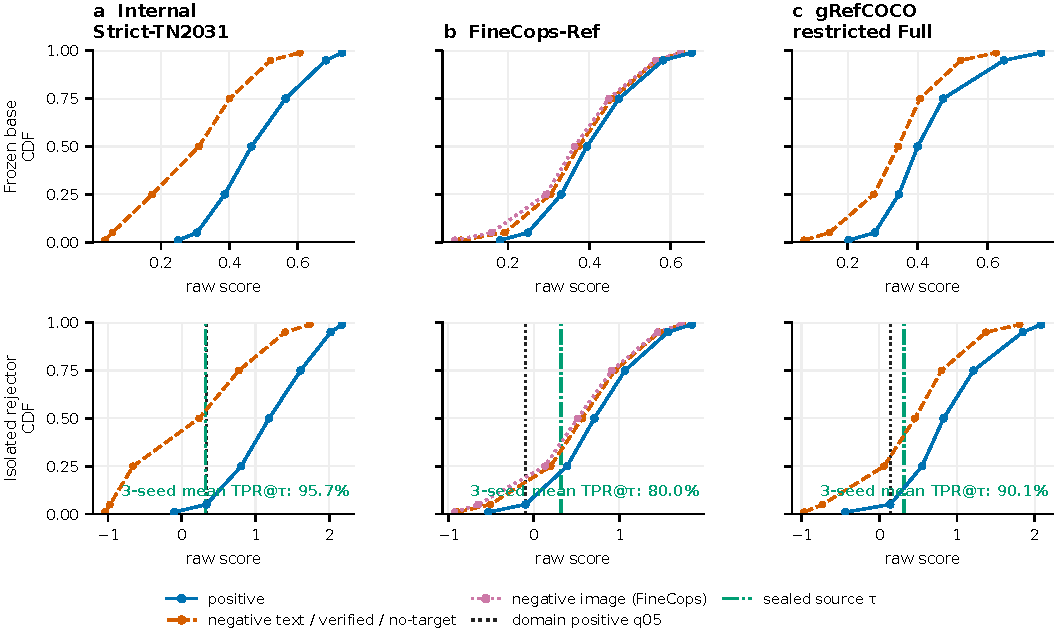
\includegraphics[width=\textwidth]{supplement/figures/figS1_confidence_anatomy.pdf}
  \caption{Confidence anatomy across the internal, FineCops-Ref, and
  restricted gRefCOCO surfaces.  Each curve samples the empirical score CDF
  at the committed 1/5/25/50/75/95/99 percentiles; the upper row is the frozen
  base and the lower row is the isolated rejector at seed 42.  The dotted
  black line is each domain's positive q05, which defines diagnostic FPR95.
  The green dash--dot line is the distinct operating threshold $\tau$ sealed
  on the 1,570-row internal calibration surface.  Its three-seed mean TPR
  remains near 95\% internally but falls on both external benchmarks.  The
  FineCops receipt seals negative-text and negative-image distributions, but
  not object/attribute/relation/swap score distributions; we therefore do not
  reconstruct unregistered subgroup curves.}
  \label{fig:sup-confidence-anatomy}
\end{figure*}

Figure~\ref{fig:sup-confidence-anatomy} separates two notions that a single
FPR95 number can obscure.  Recomputed domain q05 thresholds expose improved
positive--negative ordering, whereas the unchanged source $\tau$ exposes the
operating-point shift.  Thus external ordering gains do not imply that raw
rejector scores are calibrated probabilities or that one threshold is
universally portable.

\begin{figure*}[t]
  \centering
  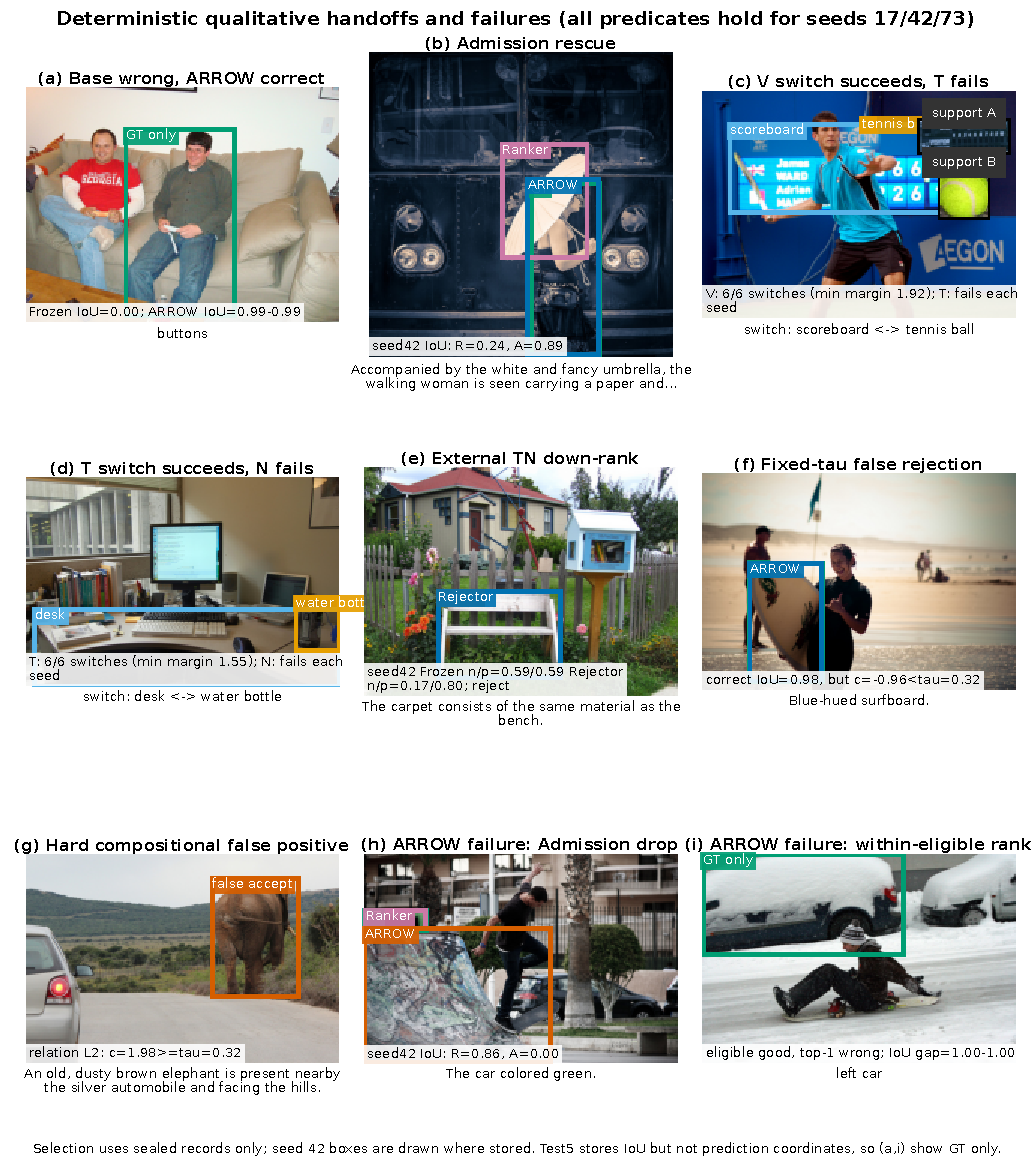
\includegraphics[width=\textwidth]{qualitative/qualitative_appendix_grid.pdf}
  \caption{Nine deterministic qualitative cases selected from sealed records.
  The predicates cover base-to-ARROW rescue, learned Admission, visual/text/null
  category switching, external rejection, fixed-threshold shift, a hard
  compositional false positive, and two honest failures.  Every predicate must
  hold for seeds 17/42/73.  Panels sourced from Test5 draw ground truth only
  because the sealed records contain IoU but not prediction coordinates; no box
  is reconstructed.}
  \label{fig:supp-qualitative}
\end{figure*}
